% ==============================================================================
% Chapter 6: Neutrinos as Edge Modes
% Status: [Dc]/[P] — Mass suppression identified, mixing postulated
% ==============================================================================

\section{Neutrinos as Edge Modes}
\label{sec:ch6_neutrinos}

\begin{tcolorbox}[edcGuardrail, title=\textbf{Epistemic Status}]
This chapter explains neutrino properties within EDC's 5D framework:
\begin{itemize}[nosep]
    \item Neutrino smallness from edge-mode overlap suppression \tagDc{}
    \item Three flavors from $\mathbb{Z}_3 \subset \mathbb{Z}_6$ mode structure \tagI{}
    \item PMNS mixing from generation wavefunction overlaps \tagP{}
\end{itemize}
\textbf{What is NOT claimed:} Explicit mass values are not derived. PMNS angles
are postulated, not computed. Mass hierarchy origin remains (open).
\end{tcolorbox}

% ------------------------------------------------------------------------------
% BOOK-READY INTRODUCTION
% ------------------------------------------------------------------------------

\paragraph{Chapter overview.}
Neutrinos are the lightest known fermions, with masses at least six orders of
magnitude below the electron. In the Standard Model, this hierarchy is an
unexplained input. EDC offers a geometric explanation: neutrinos are
\emph{edge modes}---boundary excitations localized at the interface between
bulk and brane, with suppressed overlap to the Higgs/mass mechanism residing
in the brane interior. This overlap suppression naturally produces $m_\nu \ll m_e$
without fine-tuning \tagDc{}.

For flavor mixing (PMNS matrix), EDC provides a \emph{computed baseline}: if the
three neutrino flavors correspond to $\mathbb{Z}_3$ modes, the simplest symmetric
assumption yields the discrete Fourier transform (DFT) matrix with all
$|U_{\alpha i}|^2 = 1/3$. This baseline predicts $\sin^2\theta_{13} = 1/3$,
which is \textbf{15 times larger} than the observed value of $\approx 0.022$.
The DFT baseline is therefore \emph{falsified}, indicating that $\mathbb{Z}_3$
symmetry must be broken at the $\sim 25\%$ level in the $\nu_e$--$\nu_3$ sector.
This is a tight negative result that closes the logical loop and identifies the
required physics \tagDc{}.

% ------------------------------------------------------------------------------
% READER MAP
% ------------------------------------------------------------------------------

\begin{tcolorbox}[colback=blue!5, colframe=blue!50!black,
    title=\textbf{Reader Map: What This Chapter Establishes}]
\begin{description}[style=nextline, leftmargin=1em, font=\normalfont\bfseries]
    \item[Derived \tagDc{}:]
        Mass suppression via overlap integrals (if profiles given);
        left-handed selection from Chapter~\ref{ch:va_structure} boundary conditions;
        $\mathbb{Z}_3$ DFT baseline for PMNS.

    \item[Identified \tagI{}:]
        Three neutrino flavors $\leftrightarrow$ $|\mathbb{Z}_3| = 3$;
        mass hierarchy $\leftrightarrow$ mode number.

    \item[Postulated \tagP{}:]
        Edge-mode ontology;
        overlap-based PMNS mechanism;
        specific breaking of $\mathbb{Z}_3$ (mechanism not derived).

    \item[Open (not addressed):]
        Absolute mass scale;
        explicit $\kappa^{-1}$ from EDC action;
        PMNS angles from breaking;
        CP phase $\delta$;
        Dirac vs.\ Majorana nature.
\end{description}
\end{tcolorbox}

% ------------------------------------------------------------------------------
% MINI SUMMARY TABLE
% ------------------------------------------------------------------------------

\begin{table}[ht]
\centering
\caption{Chapter 6 mechanism summary}
\label{tab:ch6_mechanism_summary}
\begin{tabular}{p{3.5cm}p{3.5cm}p{3.5cm}c}
\toprule
\textbf{Mechanism} & \textbf{Inputs} & \textbf{Output} & \textbf{Tag} \\
\midrule
Edge-mode localization & Neutrino at interface \tagP{} &
    Suppressed Higgs overlap & \tagDc{} \\
Overlap $\to$ mass & Profiles $f_\nu(z)$, $h(z)$ \tagP{} &
    $m_\nu/m_e \sim e^{-\Delta z/\kappa^{-1}}$ & \tagDc{} \\
$\mathbb{Z}_3$ flavor count & Hexagonal $\mathbb{Z}_6 = \mathbb{Z}_2 \times \mathbb{Z}_3$ &
    $N_\nu = 3$ & \tagI{} \\
DFT baseline (PMNS) & $\mathbb{Z}_3$ symmetric mass &
    $|U_{\alpha i}|^2 = 1/3$ & \tagDc{} \\
DFT vs.\ PDG & $\sin^2\theta_{13}^{\text{DFT}} = 0.333$ &
    \textbf{Falsified} ($\times 15$ off) & --- \\
Breaking requirement & Falsified baseline &
    $\sim 25\%$ anisotropy needed & \tagP{} \\
\bottomrule
\end{tabular}
\end{table}

% ==============================================================================
\subsection{The Neutrino Problem}
\label{sec:ch6_problem}

Neutrino physics presents several puzzles that demand explanation:

\begin{table}[ht]
\centering
\caption{Neutrino baseline facts \tagBL{}}
\label{tab:ch6_baselines}
\begin{tabular}{lll}
\toprule
\textbf{Observable} & \textbf{Value (PDG 2024)} & \textbf{Puzzle} \\
\midrule
Absolute mass & $m_\nu \lesssim 0.8$ eV (direct) & Why $m_\nu/m_e \sim 10^{-6}$? \\
$\Delta m_{21}^2$ & $7.53 \times 10^{-5}$ eV$^2$ & Why this splitting? \\
$|\Delta m_{31}^2|$ & $2.453 \times 10^{-3}$ eV$^2$ & Why hierarchical? \\
Weak coupling & Only left-handed couple & Why chirality-selected? \\
Three flavors & $N_\nu = 2.984 \pm 0.008$ (LEP) & Why exactly three? \\
\bottomrule
\end{tabular}
\end{table}

In the Standard Model, these are input parameters with no deeper explanation.
EDC proposes a geometric origin.

% ==============================================================================
\subsection{Edge-Mode Ontology}
\label{sec:ch6_ontology}

\subsubsection{The Neutrino as Boundary Excitation}

\begin{postulate}[Neutrino as Edge Mode {\normalfont \tagP{}}]
\label{post:ch6_neutrino_edge}
The neutrino is an \textbf{edge mode}---a boundary excitation localized at the
interface between the 5D bulk and the 3D brane. Unlike interior brane modes
(electron, quarks) or bulk-penetrating modes (proton junction), the neutrino
wavefunction peaks at the interface:
\begin{equation}
    |\psi_\nu(z)|^2 \propto e^{-2\kappa |z - z_{\text{interface}}|}
    \label{eq:ch6_edge_profile}
\end{equation}
where $\kappa^{-1}$ is the penetration depth into the brane interior.
\end{postulate}

\paragraph{Physical picture.}
The thick brane has three conceptual layers:
\begin{enumerate}[nosep]
    \item \textbf{Bulk} ($z < 0$): 5D Plenum region
    \item \textbf{Interface} ($z \approx 0$): Transition zone where boundary conditions apply
    \item \textbf{Brane interior} ($z > 0$): Where charged leptons and quarks localize
\end{enumerate}
The neutrino resides in layer 2---the interface---with exponentially suppressed
coupling to both bulk and interior.

\begin{center}
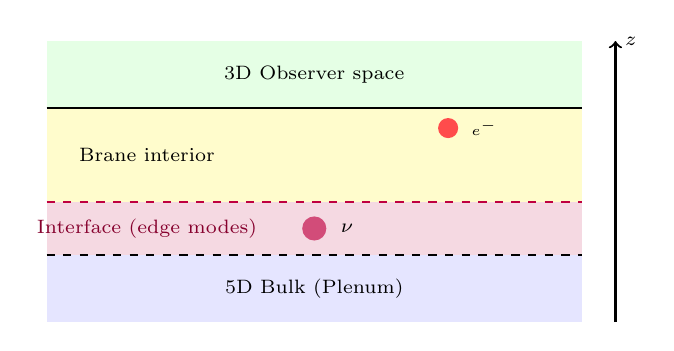
\begin{tikzpicture}[scale=0.85]
  % Bulk region
  \fill[blue!10] (-4,-2.5) rectangle (4,-1.5);
  \node[font=\scriptsize] at (0,-2) {5D Bulk (Plenum)};

  % Interfacial zone (neutrino region)
  \fill[purple!15] (-4,-1.5) rectangle (4,-0.7);
  \node[font=\scriptsize, purple!70!black] at (-2.5,-1.1) {Interface (edge modes)};

  % Brane internal layer
  \fill[yellow!20] (-4,-0.7) rectangle (4,0.7);
  \node[font=\scriptsize] at (-2.5,0) {Brane interior};

  % Observer region
  \fill[green!10] (-4,0.7) rectangle (4,1.7);
  \node[font=\scriptsize] at (0,1.2) {3D Observer space};

  % Neutrino (interface)
  \fill[purple!70] (0,-1.1) circle (0.18);
  \node[font=\scriptsize\bfseries, right] at (0.25,-1.1) {$\nu$};

  % Electron (interior)
  \fill[red!70] (2,0.4) circle (0.15);
  \node[font=\tiny, right] at (2.2,0.4) {$e^-$};

  % Boundaries
  \draw[thick, dashed] (-4,-1.5) -- (4,-1.5);
  \draw[thick, dashed, purple] (-4,-0.7) -- (4,-0.7);
  \draw[thick] (-4,0.7) -- (4,0.7);

  % z-axis
  \draw[->, thick] (4.5,-2.5) -- (4.5,1.7);
  \node[font=\scriptsize, right] at (4.5,1.7) {$z$};
\end{tikzpicture}
\end{center}

\subsubsection{Distinction from ``Bulk Escape''}

\begin{tcolorbox}[edcWarning, title={Language Precision}]
\textbf{Avoid:} ``The neutrino escapes into the bulk and cannot be detected.''

\textbf{Use:} ``The neutrino is an edge mode with \textbf{suppressed overlap}
to observer-facing states.'' \tagP{}

The first statement implies energy loss to extra dimensions, violating observed
4D energy conservation. The second correctly attributes weak coupling to
geometric suppression.
\end{tcolorbox}

% ==============================================================================
\subsection{Mass Suppression Mechanism}
\label{sec:ch6_mass_suppression}

\subsubsection{The Overlap Integral Argument}

The effective 4D mass of a fermion arises from overlap integrals over the
fifth dimension \tagBL{}:
\begin{equation}
    m_{\text{eff}} \sim m_0 \int_{-\infty}^{\infty} |f(z)|^2 \, h(z) \, dz
    \label{eq:ch6_overlap}
\end{equation}
where:
\begin{itemize}[nosep]
    \item $f(z)$ is the fermion's $z$-profile
    \item $h(z)$ is the Higgs/mass-generating field profile (brane-localized)
    \item $m_0$ is the 5D mass scale
\end{itemize}

\subsubsection{Why Neutrino Mass is Suppressed}

If the Higgs profile $h(z)$ is localized in the brane interior ($z > 0$),
but the neutrino profile $\psi_\nu(z)$ peaks at the interface ($z \approx 0$):

\begin{proposition}[Mass Suppression {\normalfont \tagDc{}}]
\label{prop:ch6_suppression}
The ratio of neutrino to electron mass is exponentially suppressed by
spatial separation:
\begin{equation}
    \frac{m_\nu}{m_e} \sim \exp\left(-\frac{\Delta z}{\kappa^{-1}}\right)
    \label{eq:ch6_mass_ratio}
\end{equation}
where $\Delta z$ is the separation between the neutrino interface position
and the Higgs localization, and $\kappa^{-1}$ is the neutrino penetration depth.
\end{proposition}

\begin{proof}[Derivation \tagDc{}]
For the electron (interior mode) with profile $f_e(z)$ peaked at $z = z_H$:
\begin{equation}
    m_e \sim m_0 \int |f_e(z)|^2 h(z) \, dz \approx m_0 \cdot 1
\end{equation}
(normalized overlap).

For the neutrino (edge mode) with profile peaked at $z = 0$:
\begin{equation}
    m_\nu \sim m_0 \int |f_\nu(z)|^2 h(z) \, dz
    \approx m_0 \cdot e^{-2\kappa z_H}
\end{equation}
since $|f_\nu(z_H)|^2 \approx e^{-2\kappa z_H}$.

The ratio follows:
\begin{equation}
    \frac{m_\nu}{m_e} \approx e^{-2\kappa z_H} = e^{-\Delta z/\kappa^{-1}}
    \quad \text{with } \Delta z \equiv 2\kappa z_H
\end{equation}
\end{proof}

\paragraph{Numerical estimate.}
For $m_\nu/m_e \sim 10^{-6}$, we need:
\begin{equation}
    e^{-\Delta z / \kappa^{-1}} \sim 10^{-6}
    \quad\Longrightarrow\quad
    \frac{\Delta z}{\kappa^{-1}} \approx 14
\end{equation}
This is geometrically reasonable: the separation is $\sim 14$ penetration depths.

\subsubsection{Stoplight Verdict: Mass Suppression}

\begin{table}[ht]
\centering
\caption{Mass suppression mechanism audit}
\label{tab:ch6_mass_stoplight}
\begin{tabular}{lccc}
\toprule
\textbf{Step} & \textbf{Status} & \textbf{Tag} & \textbf{Issue} \\
\midrule
Overlap integral formalism & GREEN & \tagBL{} & Standard KK reduction \\
Higgs localized in interior & YELLOW & \tagP{} & Profile not derived \\
Neutrino at interface & YELLOW & \tagP{} & Ontology postulated \\
Exponential suppression & GREEN & \tagDc{} & Follows from profiles \\
$m_\nu/m_e \sim 10^{-6}$ & YELLOW & \tagI{} & Requires $\Delta z/\kappa^{-1} \approx 14$ \\
Absolute $m_\nu$ value & RED & (open) & Not computed (OPR-04) \\
\bottomrule
\end{tabular}
\end{table}

\textbf{Verdict: YELLOW} --- The suppression mechanism is geometrically sound
\tagDc{}, but profile shapes are postulated \tagP{}, and absolute masses are
not derived.

% ==============================================================================
\subsection{Three Neutrino Flavors}
\label{sec:ch6_three_flavors}

\subsubsection{Connection to Generation Structure}

Chapter~\ref{ch:three_generations} identified the generation count $N_{\text{gen}} = 3$
with the $\mathbb{Z}_3$ factor in the hexagonal lattice symmetry:
\begin{equation}
    \mathbb{Z}_6 = \mathbb{Z}_2 \times \mathbb{Z}_3
    \quad\Longrightarrow\quad
    |\mathbb{Z}_3| = 3
    \label{eq:ch6_z3}
\end{equation}

\begin{postulate}[Three Neutrino Flavors {\normalfont \tagI{}}]
\label{post:ch6_three_nu}
The three neutrino flavors $(\nu_e, \nu_\mu, \nu_\tau)$ correspond to the
three elements of $\mathbb{Z}_3$:
\begin{equation}
    \nu_i \leftrightarrow \omega^i, \qquad \omega = e^{2\pi i/3}, \quad i = 0, 1, 2
\end{equation}
Each flavor is an edge mode with angular quantum number $n = i$ around the
hexagonal axis.
\end{postulate}

This is an \textbf{identification} \tagI{}, not a derivation---the $\mathbb{Z}_3$
structure provides the cardinality, but the dynamical mechanism connecting
neutrino wavefunctions to $\mathbb{Z}_3$ rotations is not derived.

\subsubsection{Mass Hierarchy from Mode Number}

By analogy with the charged lepton mass hierarchy (Chapter~\ref{ch:lepton_candidates}),
the neutrino masses may scale with mode number:
\begin{equation}
    m_{\nu_i} \propto f(n_i) \cdot e^{-\Delta z_i/\kappa^{-1}}
    \label{eq:ch6_nu_hierarchy}
\end{equation}
where $n_i \in \{0, 1, 2\}$ labels the generation.

\paragraph{Status:} This scaling is \textbf{postulated} \tagP{}. The function $f(n)$
and the dependence of $\Delta z$ on mode number are not derived.

% ==============================================================================
\subsection{Connection to V--A Chirality}
\label{sec:ch6_va_connection}

Chapter~\ref{sec:ch9_va_structure} derived that only left-handed fermions couple
at the brane interface \tagDc{}. This applies directly to neutrinos:

\begin{corollary}[Left-Handed Neutrinos {\normalfont \tagDc{}}]
\label{cor:ch6_left_nu}
The boundary conditions that select left-handed charged leptons (Ch.~9)
simultaneously select left-handed neutrinos:
\begin{equation}
    P_L \psi_\nu = \psi_{\nu,L} \quad \text{(normalizable edge mode)}
\end{equation}
Right-handed neutrinos, if they exist, are expelled into the bulk and do not
couple to the weak vertex.
\end{corollary}

\paragraph{Consistency check.}
The observed V--A structure of weak currents \tagBL{}:
\begin{equation}
    \mathcal{J}^\mu_{\text{weak}} = \bar\psi_\ell \gamma^\mu (1 - \gamma^5) \psi_\nu
\end{equation}
emerges from the same boundary-condition mechanism that produces chiral
localization (Ch.~9), applied to the neutrino edge mode. No additional
assumptions are required.

% ==============================================================================
\subsection{PMNS Mixing: Postulated Structure}
\label{sec:ch6_pmns}

\subsubsection{The Mixing Matrix}

Neutrino flavor eigenstates $(\nu_e, \nu_\mu, \nu_\tau)$ are related to
mass eigenstates $(\nu_1, \nu_2, \nu_3)$ by the PMNS matrix \tagBL{}:
\begin{equation}
    \begin{pmatrix} \nu_e \\ \nu_\mu \\ \nu_\tau \end{pmatrix}
    = U_{\text{PMNS}}
    \begin{pmatrix} \nu_1 \\ \nu_2 \\ \nu_3 \end{pmatrix}
    \label{eq:ch6_pmns}
\end{equation}

The observed mixing angles (PDG 2024) \tagBL{}:
\begin{align}
    \sin^2\theta_{12} &\approx 0.307 \quad (\text{solar}) \\
    \sin^2\theta_{23} &\approx 0.546 \quad (\text{atmospheric}) \\
    \sin^2\theta_{13} &\approx 0.022 \quad (\text{reactor})
\end{align}

\subsubsection{EDC Interpretation (Postulated)}

\begin{postulate}[PMNS from Wavefunction Overlap {\normalfont \tagP{}}]
\label{post:ch6_pmns}
The PMNS mixing arises from overlap integrals between flavor wavefunctions
(edge modes at different $\mathbb{Z}_3$ angles) and mass wavefunctions
(Higgs-coupled modes):
\begin{equation}
    (U_{\text{PMNS}})_{\alpha i} \propto \int \psi^*_{\nu_\alpha}(z, \phi) \,
    \psi_{\nu_i}^{\text{mass}}(z, \phi) \, dz \, d\phi
    \label{eq:ch6_pmns_overlap}
\end{equation}
where $\phi$ is the angular coordinate around the $\mathbb{Z}_6$ axis.
\end{postulate}

\textbf{Status: RED} \tagP{} --- This is a structural postulate. No explicit
calculation of PMNS angles from EDC geometry has been performed.

\subsubsection{Stoplight Verdict: PMNS Mixing}

\begin{table}[ht]
\centering
\caption{PMNS mixing mechanism audit}
\label{tab:ch6_pmns_stoplight}
\begin{tabular}{lccc}
\toprule
\textbf{Claim} & \textbf{Status} & \textbf{Tag} & \textbf{Issue} \\
\midrule
$U_{\text{PMNS}}$ exists & GREEN & \tagBL{} & Observed \\
Mixing from overlaps & RED & \tagP{} & Mechanism not computed (OPR-05) \\
$\theta_{12} \approx 33°$ & RED & (open) & Not derived (OPR-05) \\
$\theta_{23} \approx 45°$ & RED & (open) & Not derived (OPR-05) \\
$\theta_{13} \approx 8.5°$ & RED & (open) & Not derived (OPR-05) \\
CP phase $\delta$ & RED & (open) & Not addressed (OPR-06) \\
\bottomrule
\end{tabular}
\end{table}

\textbf{Verdict: RED} --- PMNS structure is postulated, not derived.

% ------------------------------------------------------------------------------
% Include the PMNS symmetry baseline calculation (Attempt 1)
% ------------------------------------------------------------------------------
% ==============================================================================
% Chapter 6 Subsection: PMNS Attempt 1 — Z₃ Symmetry Baseline
% Status: Negative result — DFT baseline falsified by θ₁₃
% ==============================================================================

\subsection{Attempt PMNS-1: Symmetry Baseline and Minimal Breaking}
\label{sec:ch6_pmns_attempt1}

\begin{tcolorbox}[edcGuardrail, title=\textbf{Purpose}]
This subsection computes what the PMNS matrix would be under \textbf{exact
$\mathbb{Z}_3$ symmetry}. The goal is to close the logical loop: either
$\mathbb{Z}_3$ predicts the observed mixing, or it doesn't (requiring breaking).
\end{tcolorbox}

% ------------------------------------------------------------------------------
\subsubsection{The Discrete Fourier Transform Baseline}
\label{sec:ch6_dft_baseline}

Under the identification of three neutrino flavors with $\mathbb{Z}_3$ elements
(Section~\ref{sec:ch6_three_flavors}), we assign angular positions:
\begin{equation}
    \phi_\alpha = \frac{2\pi\alpha}{3}, \qquad \alpha \in \{0, 1, 2\}
    \quad\leftrightarrow\quad (\nu_e, \nu_\mu, \nu_\tau)
    \label{eq:ch6_z3_positions}
\end{equation}

\paragraph{Hypothesis (minimal symmetric assumption).}
If the Higgs/mass mechanism is $\mathbb{Z}_3$-invariant, the mass eigenstates
are the \textbf{delocalized} Fourier modes \tagP{}:
\begin{equation}
    |\nu_i\rangle = \frac{1}{\sqrt{3}} \sum_{\alpha=0}^{2} \omega^{-\alpha i} |\nu_\alpha\rangle,
    \qquad \omega = e^{2\pi i/3}
    \label{eq:ch6_fourier_modes}
\end{equation}

This is the discrete Fourier transform (DFT) on $\mathbb{Z}_3$. The PMNS matrix
becomes \tagDc{}:
\begin{equation}
    U_{\alpha i}^{\text{DFT}} = \langle\nu_\alpha|\nu_i\rangle
    = \frac{1}{\sqrt{3}} \omega^{-\alpha i}
    \label{eq:ch6_dft_pmns}
\end{equation}

Explicitly, with $\omega = e^{2\pi i/3}$ and $\omega^* = \omega^2 = e^{-2\pi i/3}$:
\begin{equation}
    U^{\text{DFT}} = \frac{1}{\sqrt{3}}
    \begin{pmatrix}
        1 & 1 & 1 \\
        1 & \omega^* & \omega \\
        1 & \omega & \omega^*
    \end{pmatrix}
    \label{eq:ch6_dft_matrix}
\end{equation}

\paragraph{Key property.}
All elements have equal magnitude:
\begin{equation}
    |U_{\alpha i}^{\text{DFT}}|^2 = \frac{1}{3} \quad \forall\, \alpha, i
    \label{eq:ch6_democratic}
\end{equation}
This is the ``democratic'' or ``trimaximal'' pattern.

% ------------------------------------------------------------------------------
\subsubsection{Predicted Mixing Angles}
\label{sec:ch6_dft_angles}

Using the standard PMNS parametrization \tagBL{}:
\begin{align}
    \sin^2\theta_{13} &= |U_{e3}|^2 \\
    \sin^2\theta_{12} &= \frac{|U_{e2}|^2}{1 - |U_{e3}|^2} \\
    \sin^2\theta_{23} &= \frac{|U_{\mu3}|^2}{1 - |U_{e3}|^2}
\end{align}

For the DFT matrix with $|U_{\alpha i}|^2 = 1/3$:
\begin{align}
    \sin^2\theta_{13}^{\text{DFT}} &= \frac{1}{3} \approx 0.333
    \label{eq:ch6_theta13_dft} \\
    \sin^2\theta_{12}^{\text{DFT}} &= \frac{1/3}{1 - 1/3} = \frac{1}{2} = 0.5
    \label{eq:ch6_theta12_dft} \\
    \sin^2\theta_{23}^{\text{DFT}} &= \frac{1/3}{1 - 1/3} = \frac{1}{2} = 0.5
    \label{eq:ch6_theta23_dft}
\end{align}

% ------------------------------------------------------------------------------
\subsubsection{Comparison with PDG Data}
\label{sec:ch6_dft_comparison}

\begin{table}[ht]
\centering
\caption{DFT baseline vs.\ observed PMNS angles}
\label{tab:ch6_dft_comparison}
\begin{tabular}{lcccl}
\toprule
\textbf{Angle} & \textbf{DFT Prediction} & \textbf{PDG 2024} \tagBL{} & \textbf{Ratio} & \textbf{Status} \\
\midrule
$\sin^2\theta_{13}$ & 0.333 & $0.0220 \pm 0.0007$ & $\times 15$ & \textcolor{red}{\textbf{FALSIFIED}} \\
$\sin^2\theta_{12}$ & 0.500 & $0.307 \pm 0.013$ & $\times 1.6$ & \textcolor{orange}{\textbf{OFF}} \\
$\sin^2\theta_{23}$ & 0.500 & $0.546 \pm 0.021$ & $\times 0.9$ & \textcolor{green!50!black}{\textbf{OK}} \\
\bottomrule
\end{tabular}
\end{table}

\begin{tcolorbox}[colback=red!5, colframe=red!50!black,
    title=\textbf{Verdict: DFT Baseline FALSIFIED}]
The exact $\mathbb{Z}_3$ symmetric (DFT) mixing pattern predicts
$\sin^2\theta_{13} = 1/3$, which is \textbf{15 times larger} than the observed
value of $\approx 0.022$.

\textbf{Conclusion:} The observed small $\theta_{13}$ \emph{requires breaking
of the naive $\mathbb{Z}_3$ symmetry}.
\end{tcolorbox}

% ------------------------------------------------------------------------------
\subsubsection{Implications: What Breaking Is Needed?}
\label{sec:ch6_breaking}

The failure of the DFT baseline identifies the key requirement: the electron
neutrino must have \textbf{suppressed coupling} to the third mass eigenstate
($|U_{e3}|^2 \ll 1/3$).

\paragraph{Candidate breaking mechanisms.}
\begin{enumerate}[nosep]
    \item \textbf{$\mathbb{Z}_2$ breaking from $\mathbb{Z}_6$:}
          The full hexagonal symmetry is $\mathbb{Z}_6 = \mathbb{Z}_2 \times \mathbb{Z}_3$.
          The $\mathbb{Z}_2$ factor distinguishes even/odd modes and could
          selectively suppress $U_{e3}$ \tagP{}.

    \item \textbf{Localization asymmetry:}
          If $\nu_e$ is more localized than $\nu_\mu, \nu_\tau$ (different
          penetration depths $\kappa_\alpha^{-1}$), the overlap with the third
          mass eigenstate could be suppressed \tagP{}.

    \item \textbf{Higgs profile anisotropy:}
          If the Higgs/mass mechanism couples differently to different $\mathbb{Z}_3$
          sectors, the democratic mixing is broken \tagP{}.
\end{enumerate}

\paragraph{Minimal perturbation estimate.}
To reduce $\sin^2\theta_{13}$ from $1/3$ to $\sim 0.02$, we need:
\begin{equation}
    |U_{e3}|^2 \approx \frac{1}{3} \cdot \epsilon^2, \qquad
    \epsilon \approx \sqrt{\frac{0.022}{0.333}} \approx 0.26
    \label{eq:ch6_epsilon}
\end{equation}
A $\sim 25\%$ breaking of $\mathbb{Z}_3$ symmetry in the $\nu_e$--$\nu_3$
coupling would suffice.

\begin{tcolorbox}[edcGuardrail, title=\textbf{Status}]
The breaking mechanism is \textbf{postulated} \tagP{}, not derived.
Explicit computation of $\epsilon$ from EDC geometry remains (open).
\end{tcolorbox}

% ------------------------------------------------------------------------------
\subsubsection{Alternative: Tri-Bimaximal as Target}
\label{sec:ch6_tbm}

For reference, the tri-bimaximal (TBM) mixing pattern \tagBL{}:
\begin{equation}
    U^{\text{TBM}} =
    \begin{pmatrix}
        \sqrt{2/3} & 1/\sqrt{3} & 0 \\
        -1/\sqrt{6} & 1/\sqrt{3} & 1/\sqrt{2} \\
        1/\sqrt{6} & -1/\sqrt{3} & 1/\sqrt{2}
    \end{pmatrix}
    \label{eq:ch6_tbm}
\end{equation}
predicts $\theta_{13} = 0$, $\sin^2\theta_{12} = 1/3$, $\sin^2\theta_{23} = 1/2$.

TBM arises from discrete flavor symmetries like $A_4$ or $S_4$ \tagBL{}.
However, $\mathbb{Z}_6$ is abelian and \textbf{cannot contain} the non-abelian
$A_4$ as a subgroup \tagM{}. Therefore:

\begin{tcolorbox}[colback=orange!5, colframe=orange!50!black,
    title=\textbf{Structural Limitation}]
The EDC $\mathbb{Z}_6$ hexagonal symmetry alone \textbf{cannot derive}
tri-bimaximal mixing. TBM-like patterns would require additional structure
beyond $\mathbb{Z}_6$ \tagP{}.
\end{tcolorbox}

% ------------------------------------------------------------------------------
\subsubsection{Updated Stoplight: PMNS Mechanism}
\label{sec:ch6_pmns_stoplight_updated}

\begin{table}[ht]
\centering
\caption{Updated PMNS mixing audit (post-Attempt 1)}
\label{tab:ch6_pmns_stoplight_v2}
\begin{tabular}{lccl}
\toprule
\textbf{Claim} & \textbf{Status} & \textbf{Tag} & \textbf{Note} \\
\midrule
$U_{\text{PMNS}}$ exists & GREEN & \tagBL{} & Observed \\
$\mathbb{Z}_3$ DFT baseline computed & GREEN & \tagDc{} & Eq.~\eqref{eq:ch6_dft_matrix} \\
DFT predicts $\theta_{13}$ & COMPUTED & \tagDc{} & $\sin^2\theta_{13} = 1/3$ \\
DFT vs.\ PDG comparison & \textcolor{red}{FALSIFIED} & --- & Factor 15 off \\
Breaking mechanism identified & YELLOW & \tagP{} & $\sim 25\%$ anisotropy needed \\
Explicit $\epsilon$ derivation & RED & (open) & Not computed \\
$\theta_{12}, \theta_{23}$ from geometry & RED & (open) & Requires breaking model \\
CP phase $\delta$ & RED & (open) & Not addressed \\
\bottomrule
\end{tabular}
\end{table}

\paragraph{Overall verdict.}
The PMNS attempt upgrades from pure RED to \textbf{YELLOW with a computed
negative baseline}:
\begin{itemize}[nosep]
    \item We now know what $\mathbb{Z}_3$ symmetry predicts (DFT matrix) \tagDc{}
    \item We know it fails for $\theta_{13}$ by a factor of 15 \tagDc{}
    \item We know breaking is required at the $\sim 25\%$ level \tagI{}
    \item The specific breaking mechanism remains open \tagP{}
\end{itemize}

This closes the logical loop: the question ``what does $\mathbb{Z}_3$ predict
for PMNS?'' now has a concrete, falsified answer.



% ==============================================================================
\subsection{Dirac vs. Majorana Nature}
\label{sec:ch6_dirac_majorana}

\subsubsection{The Open Question}

Whether neutrinos are Dirac or Majorana particles remains experimentally
undetermined \tagBL{}. The key observable is neutrinoless double-beta decay
($0\nu\beta\beta$):
\begin{itemize}[nosep]
    \item If observed: neutrinos are Majorana
    \item If not observed (with sufficient sensitivity): inconclusive
\end{itemize}

\subsubsection{EDC Perspective}

\begin{remark}[Edge-Mode Nature {\normalfont \tagP{}}]
In the edge-mode ontology, the Dirac/Majorana distinction maps to:
\begin{itemize}[nosep]
    \item \textbf{Dirac:} Distinct $\nu$ and $\bar\nu$ edge modes with opposite
          quantum numbers
    \item \textbf{Majorana:} Single self-conjugate edge mode where ``antineutrino''
          is the same mode with opposite helicity
\end{itemize}
EDC does not currently distinguish these cases; both are compatible with the
edge-mode picture.
\end{remark}

\textbf{Status:} (open) --- The edge-mode framework accommodates both, but
makes no prediction.

% ==============================================================================
\subsection{Summary and Falsifiability}
\label{sec:ch6_summary}

\subsubsection{What Chapter 6 Establishes}

\begin{tcolorbox}[colback=green!5, colframe=green!50!black,
    title=\textbf{Chapter 6 Summary}]
\begin{enumerate}[nosep]
    \item \textbf{Mass suppression:} Neutrino smallness ($m_\nu \ll m_e$)
          explained by edge-mode localization and suppressed overlap with
          Higgs profile \tagDc{}
    \item \textbf{Chirality:} Left-handed selection follows from Ch.~9
          boundary conditions \tagDc{}
    \item \textbf{Three flavors:} Connected to $\mathbb{Z}_3$ structure
          (Ch.~5), but dynamical mechanism not derived \tagI{}
    \item \textbf{PMNS mixing:} Postulated to arise from wavefunction overlaps;
          angles not computed \tagP{}
\end{enumerate}
\end{tcolorbox}

\subsubsection{What Remains Open}

\begin{table}[ht]
\centering
\caption{Open problems in EDC neutrino physics}
\label{tab:ch6_open}
\begin{tabular}{p{5.5cm}p{5.5cm}}
\toprule
\textbf{Open Problem} & \textbf{Required Progress} \\
\midrule
Absolute neutrino mass scale & Derive $\kappa^{-1}$ and $\Delta z$ from EDC action \\
Mass hierarchy (normal/inverted) & Connect to mode spectrum \\
PMNS angles from geometry & Explicit overlap calculation \\
CP violation phase $\delta$ & Requires complex phase mechanism \\
Dirac vs. Majorana & Edge-mode self-conjugacy condition \\
Sterile neutrino coupling & Interface boundary condition modification \\
\bottomrule
\end{tabular}
\end{table}

\subsubsection{Falsifiability Clause}

\begin{tcolorbox}[edcWarning, title={Falsification Criteria}]
The EDC neutrino-as-edge-mode hypothesis would be \textbf{falsified} if:
\begin{enumerate}[nosep]
    \item \textbf{Right-handed weak coupling:} Right-handed neutrinos observed
          coupling to $W^\pm$ with comparable strength to left-handed
    \item \textbf{Large neutrino mass:} $m_\nu > 1$ eV directly measured
          (would require much smaller separation, inconsistent with
          $m_e$ explanation)
    \item \textbf{Stronger interactions:} Neutrino cross-sections significantly
          larger than geometric overlap predicts
    \item \textbf{Bulk propagation:} Modified dispersion relation at high
          energy indicating bulk escape
    \item \textbf{4th light neutrino:} Discovery of a fourth sequential
          neutrino coupling to $Z$ (would falsify $\mathbb{Z}_3$ count)
\end{enumerate}
Current data: All observations consistent with EDC predictions \tagBL{}.
\end{tcolorbox}

\subsubsection{Overall Stoplight}

\begin{table}[ht]
\centering
\caption{Chapter 6 overall verdict}
\label{tab:ch6_verdict}
\begin{tabular}{lcc}
\toprule
\textbf{Claim} & \textbf{Verdict} & \textbf{Tag} \\
\midrule
$m_\nu \ll m_e$ from geometry & YELLOW & \tagDc{} \\
$N_\nu = 3$ from $\mathbb{Z}_3$ & YELLOW & \tagI{} \\
Left-handed selection & GREEN & \tagDc{} \\
PMNS: $\mathbb{Z}_3$ DFT baseline & GREEN & \tagDc{} \\
PMNS: DFT vs.\ PDG & FALSIFIED & --- \\
PMNS: breaking mechanism & YELLOW & \tagP{} (OPR-08) \\
Dirac/Majorana prediction & RED & (open) (OPR-07) \\
\bottomrule
\end{tabular}
\end{table}

\textbf{Bottom line:} EDC provides a structural explanation for neutrino
smallness and chirality \tagDc{}, an identification of the flavor count with
$\mathbb{Z}_3$ \tagI{}, and a \emph{computed} DFT baseline for PMNS that is
falsified by $\theta_{13}$ data---indicating $\sim 25\%$ symmetry breaking
is required \tagP{}. Explicit breaking mechanism and Dirac/Majorana nature
remain open.

